

\tikzset{every picture/.style={line width=0.5pt}} %set default line width to 0.75pt        

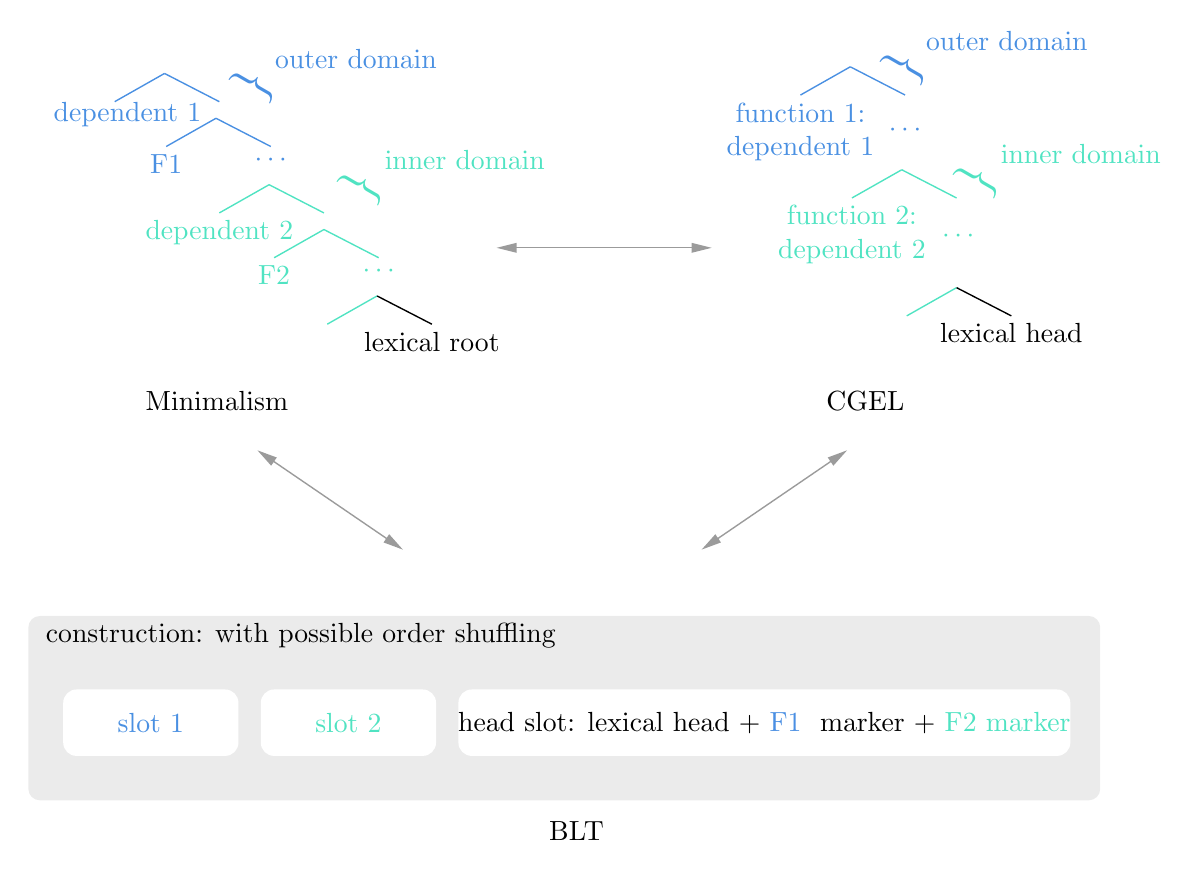
\begin{tikzpicture}[x=0.75pt,y=0.75pt,yscale=-0.8,xscale=0.8]
%uncomment if require: \path (0,559); %set diagram left start at 0, and has height of 559

%Straight Lines [id:da5621104818803937] 
\draw [color={rgb, 255:red, 80; green, 227; blue, 194 }  ,draw opacity=1 ]   (226,174) -- (256,157) ;
%Straight Lines [id:da8460516076186504] 
\draw [color={rgb, 255:red, 80; green, 227; blue, 194 }  ,draw opacity=1 ]   (289,174) -- (256,157) ;
%Straight Lines [id:da8167707353848563] 
\draw [color={rgb, 255:red, 80; green, 227; blue, 194 }  ,draw opacity=1 ]   (258,214) -- (288,197) ;
%Straight Lines [id:da97843300736648] 
\draw    (321,214) -- (288,197) ;
%Straight Lines [id:da5814349351958874] 
\draw [color={rgb, 255:red, 74; green, 144; blue, 226 }  ,draw opacity=1 ]   (161,107) -- (168.67,102.65) -- (191,90) ;
%Straight Lines [id:da9675905225272661] 
\draw [color={rgb, 255:red, 74; green, 144; blue, 226 }  ,draw opacity=1 ]   (224,107) -- (191,90) ;
%Straight Lines [id:da0412318007492094] 
\draw [color={rgb, 255:red, 80; green, 227; blue, 194 }  ,draw opacity=1 ]   (574,138) -- (604,121) ;
%Straight Lines [id:da7765915673023971] 
\draw [color={rgb, 255:red, 80; green, 227; blue, 194 }  ,draw opacity=1 ]   (637,138) -- (604,121) ;
%Straight Lines [id:da3903934581615822] 
\draw [color={rgb, 255:red, 80; green, 227; blue, 194 }  ,draw opacity=1 ]   (607,209) -- (637,192) ;
%Straight Lines [id:da8557785144848347] 
\draw    (670,209) -- (637,192) ;
%Straight Lines [id:da16499526186432512] 
\draw [color={rgb, 255:red, 74; green, 144; blue, 226 }  ,draw opacity=1 ]   (543,76) -- (550.67,71.65) -- (573,59) ;
%Straight Lines [id:da4544217016044618] 
\draw [color={rgb, 255:red, 74; green, 144; blue, 226 }  ,draw opacity=1 ]   (606,76) -- (573,59) ;
%Straight Lines [id:da9960388692953916] 
\draw [color={rgb, 255:red, 80; green, 227; blue, 194 }  ,draw opacity=1 ]   (193,147) -- (223,130) ;
%Straight Lines [id:da42039690968517274] 
\draw [color={rgb, 255:red, 80; green, 227; blue, 194 }  ,draw opacity=1 ]   (256,147) -- (223,130) ;
%Straight Lines [id:da7930646382251649] 
\draw [color={rgb, 255:red, 74; green, 144; blue, 226 }  ,draw opacity=1 ]   (130,80) -- (137.67,75.65) -- (160,63) ;
%Straight Lines [id:da560139439993615] 
\draw [color={rgb, 255:red, 74; green, 144; blue, 226 }  ,draw opacity=1 ]   (193,80) -- (160,63) ;
%Straight Lines [id:da2026063761389032] 
\draw [color={rgb, 255:red, 155; green, 155; blue, 155 }  ,draw opacity=1 ]   (362,168) -- (487.51,168) ;
\draw [shift={(489.51,168)}, rotate = 180] [fill={rgb, 255:red, 155; green, 155; blue, 155 }  ,fill opacity=1 ][line width=0.08]  [draw opacity=0] (12,-3) -- (0,0) -- (12,3) -- cycle    ;
\draw [shift={(360,168)}, rotate = 0] [fill={rgb, 255:red, 155; green, 155; blue, 155 }  ,fill opacity=1 ][line width=0.08]  [draw opacity=0] (12,-3) -- (0,0) -- (12,3) -- cycle    ;
%Rounded Rect [id:dp4576906617870975] 
\draw  [draw opacity=0][fill={rgb, 255:red, 155; green, 155; blue, 155 }  ,fill opacity=0.2 ] (78,396.63) .. controls (78,392.82) and (81.08,389.74) .. (84.89,389.74) -- (716.62,389.74) .. controls (720.42,389.74) and (723.51,392.82) .. (723.51,396.63) -- (723.51,493.85) .. controls (723.51,497.66) and (720.42,500.74) .. (716.62,500.74) -- (84.89,500.74) .. controls (81.08,500.74) and (78,497.66) .. (78,493.85) -- cycle ;
%Rounded Rect [id:dp4322477894173522] 
\draw  [draw opacity=0][fill={rgb, 255:red, 255; green, 255; blue, 255 }  ,fill opacity=1 ] (99,442) .. controls (99,437.58) and (102.58,434) .. (107,434) -- (196.51,434) .. controls (200.93,434) and (204.51,437.58) .. (204.51,442) -- (204.51,466) .. controls (204.51,470.42) and (200.93,474) .. (196.51,474) -- (107,474) .. controls (102.58,474) and (99,470.42) .. (99,466) -- cycle ;
%Rounded Rect [id:dp5387240226143777] 
\draw  [draw opacity=0][fill={rgb, 255:red, 255; green, 255; blue, 255 }  ,fill opacity=1 ] (218,442) .. controls (218,437.58) and (221.58,434) .. (226,434) -- (315.51,434) .. controls (319.93,434) and (323.51,437.58) .. (323.51,442) -- (323.51,466) .. controls (323.51,470.42) and (319.93,474) .. (315.51,474) -- (226,474) .. controls (221.58,474) and (218,470.42) .. (218,466) -- cycle ;
%Straight Lines [id:da32838392012871354] 
\draw [color={rgb, 255:red, 155; green, 155; blue, 155 }  ,draw opacity=1 ]   (217.65,291.13) -- (301.86,348.61) ;
\draw [shift={(303.51,349.74)}, rotate = 214.32] [fill={rgb, 255:red, 155; green, 155; blue, 155 }  ,fill opacity=1 ][line width=0.08]  [draw opacity=0] (12,-3) -- (0,0) -- (12,3) -- cycle    ;
\draw [shift={(216,290)}, rotate = 34.32] [fill={rgb, 255:red, 155; green, 155; blue, 155 }  ,fill opacity=1 ][line width=0.08]  [draw opacity=0] (12,-3) -- (0,0) -- (12,3) -- cycle    ;
%Straight Lines [id:da7435418496058712] 
\draw [color={rgb, 255:red, 155; green, 155; blue, 155 }  ,draw opacity=1 ]   (569.36,291.13) -- (485.16,348.61) ;
\draw [shift={(483.51,349.74)}, rotate = 325.68] [fill={rgb, 255:red, 155; green, 155; blue, 155 }  ,fill opacity=1 ][line width=0.08]  [draw opacity=0] (12,-3) -- (0,0) -- (12,3) -- cycle    ;
\draw [shift={(571.02,290)}, rotate = 145.68] [fill={rgb, 255:red, 155; green, 155; blue, 155 }  ,fill opacity=1 ][line width=0.08]  [draw opacity=0] (12,-3) -- (0,0) -- (12,3) -- cycle    ;
%Rounded Rect [id:dp3559533888781332] 
\draw  [draw opacity=0][fill={rgb, 255:red, 255; green, 255; blue, 255 }  ,fill opacity=1 ] (337,442) .. controls (337,437.58) and (340.58,434) .. (345,434) -- (697.51,434) .. controls (701.93,434) and (705.51,437.58) .. (705.51,442) -- (705.51,466) .. controls (705.51,470.42) and (701.93,474) .. (697.51,474) -- (345,474) .. controls (340.58,474) and (337,470.42) .. (337,466) -- cycle ;

% Text Node
\draw (321,217) node [anchor=north] [inner sep=0.75pt]   [align=left] {lexical root};
% Text Node
\draw (225,46.85) node [anchor=north west][inner sep=0.75pt]  [color={rgb, 255:red, 74; green, 144; blue, 226 }  ,opacity=1 ] [align=left] {outer domain};
% Text Node
\draw (291,107.85) node [anchor=north west][inner sep=0.75pt]  [color={rgb, 255:red, 80; green, 227; blue, 194 }  ,opacity=1 ] [align=left] {inner domain};
% Text Node
\draw (161,110) node [anchor=north] [inner sep=0.75pt]  [color={rgb, 255:red, 74; green, 144; blue, 226 }  ,opacity=1 ] [align=left] {F1};
% Text Node
\draw (226,177) node [anchor=north] [inner sep=0.75pt]  [color={rgb, 255:red, 80; green, 227; blue, 194 }  ,opacity=1 ] [align=left] {F2};
% Text Node
\draw (147,253) node [anchor=north west][inner sep=0.75pt]   [align=left] {Minimalism};
% Text Node
\draw (670,212) node [anchor=north] [inner sep=0.75pt]   [align=left] {lexical head};
% Text Node
\draw (543,79) node [anchor=north] [inner sep=0.75pt]  [color={rgb, 255:red, 74; green, 144; blue, 226 }  ,opacity=1 ] [align=left] {\begin{minipage}[lt]{57.06pt}\setlength\topsep{0pt}
\begin{center}
function 1:\\dependent 1\\
\end{center}

\end{minipage}};
% Text Node
\draw (574,141) node [anchor=north] [inner sep=0.75pt]  [color={rgb, 255:red, 80; green, 227; blue, 194 }  ,opacity=1 ] [align=left] {\begin{minipage}[lt]{57.06pt}\setlength\topsep{0pt}
\begin{center}
function 2:\\dependent 2
\end{center}

\end{minipage}};
% Text Node
\draw (193,150) node [anchor=north] [inner sep=0.75pt]  [color={rgb, 255:red, 80; green, 227; blue, 194 }  ,opacity=1 ] [align=left] {dependent 2};
% Text Node
\draw (137.67,78.65) node [anchor=north] [inner sep=0.75pt]  [color={rgb, 255:red, 74; green, 144; blue, 226 }  ,opacity=1 ] [align=left] {dependent 1};
% Text Node
\draw (224,110) node [anchor=north] [inner sep=0.75pt]  [color={rgb, 255:red, 74; green, 144; blue, 226 }  ,opacity=1 ] [align=left] {$\displaystyle \cdots $};
% Text Node
\draw (289,177) node [anchor=north] [inner sep=0.75pt]  [color={rgb, 255:red, 80; green, 227; blue, 194 }  ,opacity=1 ] [align=left] {$\displaystyle \cdots $};
% Text Node
\draw (606,92) node [anchor=north] [inner sep=0.75pt]  [color={rgb, 255:red, 74; green, 144; blue, 226 }  ,opacity=1 ] [align=left] {$\displaystyle \cdots $};
% Text Node
\draw (638,156) node [anchor=north] [inner sep=0.75pt]  [color={rgb, 255:red, 80; green, 227; blue, 194 }  ,opacity=1 ] [align=left] {$\displaystyle \cdots $};
% Text Node
\draw (557,252.85) node [anchor=north west][inner sep=0.75pt]   [align=left] {CGEL};
% Text Node
\draw (232.11,70.5) node [anchor=north west][inner sep=0.75pt]  [color={rgb, 255:red, 74; green, 144; blue, 226 }  ,opacity=1 ,rotate=-120] [align=left] {{\LARGE \{}};
% Text Node
\draw (297.11,131.5) node [anchor=north west][inner sep=0.75pt]  [color={rgb, 255:red, 80; green, 227; blue, 194 }  ,opacity=1 ,rotate=-120] [align=left] {{\LARGE \{}};
% Text Node
\draw (617,35.85) node [anchor=north west][inner sep=0.75pt]  [color={rgb, 255:red, 74; green, 144; blue, 226 }  ,opacity=1 ] [align=left] {outer domain};
% Text Node
\draw (662,103.85) node [anchor=north west][inner sep=0.75pt]  [color={rgb, 255:red, 80; green, 227; blue, 194 }  ,opacity=1 ] [align=left] {inner domain};
% Text Node
\draw (624.11,59.5) node [anchor=north west][inner sep=0.75pt]  [color={rgb, 255:red, 74; green, 144; blue, 226 }  ,opacity=1 ,rotate=-120] [align=left] {{\LARGE \{}};
% Text Node
\draw (668.11,127.5) node [anchor=north west][inner sep=0.75pt]  [color={rgb, 255:red, 80; green, 227; blue, 194 }  ,opacity=1 ,rotate=-120] [align=left] {{\LARGE \{}};
% Text Node
\draw (390,511.85) node [anchor=north west][inner sep=0.75pt]   [align=left] {BLT};
% Text Node
\draw (151.75,454) node  [color={rgb, 255:red, 74; green, 144; blue, 226 }  ,opacity=1 ] [align=left] {slot 1};
% Text Node
\draw (270.75,454) node  [color={rgb, 255:red, 80; green, 227; blue, 194 }  ,opacity=1 ] [align=left] {slot 2};
% Text Node
\draw (521.25,454) node  [color={rgb, 255:red, 0; green, 0; blue, 0 }  ,opacity=1 ] [align=left] {head slot: lexical head + \textcolor[rgb]{0.29,0.56,0.89}{F1} \ marker + \textcolor[rgb]{0.31,0.89,0.76}{F2 marker}};
% Text Node
\draw (86.89,392.74) node [anchor=north west][inner sep=0.75pt]   [align=left] {construction: with possible order shuffling};


\end{tikzpicture}
